\begin{titlepage}

\begin{center}

%% Extra whitespace at the top.
\vspace*{2\bigskipamount}

%% Print the title.
{\makeatletter
\titlestyle\singlespacing\bfseries\LARGE\@title\par
\makeatother}

%% Print the optional subtitle.
{\makeatletter
\ifx\@subtitle\undefined\else
    \bigskip
    \titlefont\titleshape\Large\@subtitle
\fi
\makeatother}

\end{center}

\cleardoublepage
\thispagestyle{empty}

\begin{center}

%% The following lines repeat the previous page exactly.

\vspace*{2\bigskipamount}

%% Print the title.
{\makeatletter
\titlestyle\singlespacing\bfseries\LARGE\@title\par
\makeatother}

%% Print the optional subtitle.
{\makeatletter
\ifx\@subtitle\undefined\else
    \bigskip
    \titlefont\titleshape\Large\@subtitle
\fi
\makeatother}


%% Uncomment the following lines to insert a vertically centered picture into
%% the title page.
%\vfill
%\includegraphics{title}
\vfill

%% Apart from the names and dates, the following text is dictated by the
%% promotieregelement.

{\Large\titlefont\bfseries Proefschrift}

\bigskip
\bigskip

ter verkrijging van de graad van doctor

aan de Technische Universiteit Delft,

op gezag van de Rector Magnificus prof.~dr.~ir.~T.~H.~J.~J.~van der Hagen,

voorzitter van het College voor Promoties,

in het openbaar te verdedigen op [datum] [maand] [Jaar] om [ ] uur

\bigskip
\bigskip

door

\bigskip
\bigskip

%% Print the full name of the author.
\makeatletter
{\Large\titlefont\bfseries\@firstname\ {\titleshape\@lastname}}
\makeatother
\\
\vspace{3mm}
\begin{CJK*}{UTF8}{gkai}
\makeatletter
{\LARGE\titlefont\bfseries\@lastnameCH\ \hspace{1mm} {\titleshape\@firstnameCH}}
\makeatother
\end{CJK*}

\bigskip
\bigskip

Master of Science in Applied Physics,

Technische Universiteit Delft, Nederland,

geboren te Hohhot, P.~R.~China.

%% Extra whitespace at the bottom.
\vspace*{2\bigskipamount}

\end{center}

\clearpage
\thispagestyle{empty}

%% The following line is dictated by the promotieregelement.
\noindent Dit proefschrift is goedgekeurd door de promotoren.

%% List the promotors (supervisors).
%\medskip\noindent
%\begin{tabular}{l}
%    Prof.\ dr.\ H.\ P.\ Urbach
%\end{tabular}

%% List the (optional) copromotor.
%\medskip
%\noindent Copromotor: Dr.\ F.\ Bociort

\medskip
\noindent Samenstelling promotiecommissie:

%% List the committee members, starting with the Rector Magnificus and the
%% promotor(s) and ending with the reserve members.
\medskip\noindent
\begin{tabular}{ll}
    Rector Magnificus, & voorzitter \\
    Prof.\ dr.\ H.\ P.\ Urbach, & Technische Universiteit Delft, promotor \\
    Dr.\ F.\ Bociort, & Technische Universiteit Delft, copromotor \\
\end{tabular}

\medskip
\medskip\noindent
\begin{tabular}{ll}
    \emph{Onafhankelijke leden:}\\
    ??? & ??? \\
    ??? & ??? \\
    ??? & ??? \\
    ??? & ??? \\
    ??? & ??? \\
\end{tabular}

%% Include the following disclaimer for committee members who have contributed
%% to this dissertation. Its formulation is again dictated by the
%% promotieregelement.
\medskip
\noindent Prof.\ dr.\ ir.\ ???.\ ??? heeft als begeleider in belangrijke mate aan de totstandkoming van het proefschrift bijgedragen.

%% Here you can include the logos of any institute that contributed financially
%% to this dissertation.
\vfill
\begin{center}
    
\includegraphics[height=0.6in]{title/logos/tudelftpng}
    \hspace{2em}
    
\includegraphics[height=0.6in]{title/logos/marie-curie}
    \hspace{2em}
    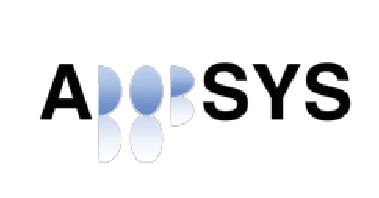
\includegraphics[height=0.55in]{title/logos/adopsys}
\end{center}
\vfill

\noindent
\begin{tabular}{@{}p{0.2\textwidth}@{}p{0.8\textwidth}}
    \textit{Keywords:} & Optical Design, Lens Design Method, Optimization, Saddle Point \\[\medskipamount]
    \textit{Printed by:} & Ipskamp Printing \\[\medskipamount]
    \textit{Front \& Back:} & Beautiful cover art that captures the entire content of this thesis in a single illustration.
\end{tabular}

\vspace{4\bigskipamount}

\noindent Copyright \textcopyright\ 2023 by Zhe Hou

%% Uncomment the following lines if this dissertation is part of the Casimir PhD
%% Series, or a similar research school.
%\medskip
%\noindent Casimir PhD Series, Delft-Leiden 2013-01

\medskip
\noindent ISBN 000-00-0000-000-0

\medskip
\noindent An electronic version of this dissertation is available at \\
\url{http://repository.tudelft.nl/}.

\newpage
\;
\vspace{12em}



% Here is the explanation about the cover
\begin{figure}[h!]
    \centering
    
\includegraphics[scale=0.35]{cover/CoverSP.png}
\end{figure} 
Designed by Hui Lin

 The concept is borrowed from Escher's style. We draw horse patterns together with the "saddle" which relates to the "saddle point". In between the horse patterns, there are pieces of convex and concave lens shape. I would like to indicate a lens design network or space that the lens solutions are linked/surrounded by saddles (saddle points). In a whole, with Escher's way of presenting, the pattern seems quite complicated, yet is composed with a monotonic repetitive pattern (the feeling of the complexity is probably from the color composition and angular arrangement). It is sort of related to the goal of the thesis/research: in a complicated design landscape, we are trying to find a systematic way to describe it and then utilize knowledge for practical design. 

\end{titlepage}

